%----------------------------------------------------------------------------
\chapter{A DeadlockHunter program}
\label{sec:dlhunter}
%----------------------------------------------------------------------------

    \section{Motiváció}
    A Morgan Stanley Magyarország Elemző Kft széles profiljának jelentős eleme az anyacég pénzügyi tevékenységének informatikai és matematikai támogatása. Számos nagyteljesítményű alkalmazást fejleszt és üzemeltet, melyek feladata a kereskedelem során generálódó adatok feldolgozása és értelmezése. Ezen rendszerek egyike egy -- tőzsdei kereskedelemhez köthető -- meglehetősen sokrétű alkalmazás hálózat, melynek fejlesztésével, karbantartásával és integrációjával foglalkoztam. A legnagyobb komponens egy C++ nyelven írt szerveroldali alkalmazás -- továbbiakban \emph{GlobalContractor} -- mely egy MIMO rendszerrel modellezhető: Sok forrásból gyűjt adatokat melyeket transzformáció után több előfizető felé publikál. A multi input-multi output modell hatákony skálázódásának biztosítása érdekében az alkalmazás folyamatosan több -- egymástól különböző feladatú, de azonos adathalmazon dolgozó -- szálat alkalmaz.
    
    Sajnálatos módon a többszálú szervezés magával von néhány kellemetlen problémát, így többször előfordult, hogy egy új komponens bevezetésekor az alkalmazás -- semmiféleképpen sem determinisztikus módon -- holtpontra jutott. A holtpont megjelenése az éles környezetben futó nagyteljesítményű szerverek esetén volt jellemző, a hibák felderítését a kereskedelmi adatok bizalmasságára vonatkozó szabályok tovább nehezítették.
    
    Egy olyan megoldásra volt szükség, ami a holtpont jellegű problémákat teljes egészében megszünteti vagy megszüntethetővé teszi, valamit bizonyosságot ad arra, hogy a vizsgált rendszer holtpontmentes -- amennyiben valójában az. Emellett követelmény volt, hogy az alkalmazás konkurens skálázódási jellemzői ne degradálódjanak, valamint a megoldás alkalmazása ne igényelje a teljes rendszer átszervezését.
    
    \section{Megoldás}
    A fentiek alapján látható, hogy az igények pontosan azt a halmazt alkotják, amit az első fejezet megoldásai nem tudnak kielégíteni. Azok a technikák, amiket a tervezés elejétől kezdve kell alkalmazni, teljes újraírást igényelnének, így nem használhatóak. A mérsékelt vagy alacsony teljesítménymutatóval jellemzett megoldások használhatatlanul lassúvá tennék a teljes alkalmazást. Az adott architektúra jellegéből fakadóan pedig a zármentes adatstruktúrák nem alkalmazhatóak hatékonyan. A korábban bemutatott megoldások nem hibásak vagy alacsonyabb rendűek; az igények túlzóak, ebben a formában nem tarthatóak, más megközelítést tesznek szükségessé.
    
    Ezt belátva relaxáljuk a feltételeket. Ha bármely fenti szempontból engednénk, az alkalmazás minősége romlana. Ebben a követelménycsapdában született meg egy olyan eszköz ötlete, mely csupán analízist végez, a rendszert magát változatlanul hagyja. A szükségletek azonosítása után megvizsgáltam, hogy nem létezik-e a piacon már elérhető, hasonló funkciójú megoldás. Egyedül az Intel® Parallel Studio XE 2013\footnote{http://software.intel.com/en-us/intel-parallel-inspector} eszközt találtam, mely állítja magáról, hogy holtpontanalízist képes végezni. A program hátránya meglehetősen borsos árán túl, hogy kizárólag Microsoft Visual Studio C Compilert és Intel C Compilert támogat, Gnu C Compilert nem, így alkalmatlan a konkrét esetben történő felhasználásra.
    
    Az alternatívák mérlegelése után a következő tervezői döntést hoztam: Az elkészítendő eszköz hajtson végre egy mérést a javítandó alkalmazáson, a mérési eredmény legyen egy jelentés, amely részletezi a megtalált holtpontokat (ill. holtpont lehetőségeket) és segíti a karbantartó programozót a hibát okozó folyamatok lokalizálásában. A holtponttal fenyegető szituációk azonosításának alapja a dinamikusan definiált zárolási sorrend megsértése. A megközelítés előnye, hogy a mérés definiálható úgy, hogy az később tetszőleges alkalmazást ki tudjon szolgálni, valamint nem, vagy csak kis mértékben igényli a mért alkalmazás módosításáát. Hátránya, hogy csak diagnosztizál, a holtponthelyzetek tényleges kiküszöbölése emberi beavatkozást igényel. A módosítás helyének megbecsülésében a mérőeszköz javaslatokkal segíti a programozót.
    
    Mivel a tervezés idejében sem a GCC AST (\emph{Abstract Syntax Tree}) plugin rendszere, sem a Clang Static Analyzere nem állt azon a szinten, hogy megfelelően támogatni tudjon egy átfogó elemzést, dinamikus kódanalízis mellett döntöttem. A dinamikus módszer szükségessé teszi a mért alkalmazás módosítását és átfogóbb tesztelést igényel, viszont a megvalósítása nagyságrendekkel egyszerűbb.
    
    A mérés formai szempontból három fázisra tagolódik: adatgyűjtés, a gyűjtött adat értelmezése és feldolgozása, eredmények megjelenítése. A következő szakaszok ezen fázisokat formalizmusát taglalják, implementációs részletek érintése nélkül.
    
    \subsection{Adatgyűjtés}
    Mivel az alkalmazásban kialakuló zárolási sorrendek felvételére van szükség, elég, ha a futás során regisztráljuk az egyes zárak egymásutániságát. A holtpontok felderítését komolyan megnehezíti, hogy azok előfordulása gyakran egy versenyhelyzet kimenetelének függvénye, a nemdeterminisztikus viselkedés nagyon megnyújtja a reprodukálásra fordítandó időt valamint nagyon körülményes arról ismételt futtatásokkal megbizonyosodni, hogy a rendszer garantáltan holtpontmentes.
    
    A \emph{deadlockHunter} nagyon fontos jellemzője, hogy a fent ismertetett bizonytalanságot kiküszöböli. Az erőforrások zárolásának és elengedésének egymásutániságát szálanként külön-külön tárolókba menti. Csak logikai sorrendet tárol, az időzítési paramétereket figyelmen kívül hagyja, így lehetővé téve azt, hogy egy későbbi fázisban a szálak egyenként rögzített aktivitását időfüggetlenül aggregáljuk.
    
    A mérés elvégzéséhez események rögzítésére van szükség. Esemény váltódik ki minden egyes alkalommal, amikor egy szál egy erőforrást zárol vagy felszabadít. Minden eseményhez logikailag két információt szükséges tárolni:
    
    \begin{description}
        \item[Esemény típusa:] Erőforrás zárolása vagy felszabadítása történt
        \item[Erőforrás azonosítása:] Bármi, ami alapján az erőforrás egyértelműen azonosítható a rendszerben, például a zár memóriacíme.
    \end{description}
%
    A \emph{deadlockHunter} ezen felül tárolja a fájlt, a metódust és a kódsort, ami az eseményt kiváltó utasítást tartalmazza, így megkönnyítve a felhasználó számára az eredmények későbbi értelmezését.
    A mérés által előállított mérési eredmény struktúrája a következőképpen formalizálható (csak a legszükségesebb jellemzőkre szorítkozva, eltekintve a később tárgyalandó implementációs részletektől): \\ \\
\texttt{Mérés: \{ Szál[] szálak \} \\
Szál: \{ Esemény[] események \} \\
Esemény: \{ EseményTípus típus, Erőforrás erőforrás \} \\
EseményTípus: boolean \\
Erőforrás: integer \\
}

    \subsection{Adatfeldolgozás}
    A fent definiált adatstruktúra feldolgozása után egy irányított $\overrightarrow{G}$ gráfot szeretnénk kapni eredményül, mely a következő képpen definiálható: $v \in V(\overrightarrow{G}) \Leftrightarrow v$ által reprezentált erőforrás a mérés folyamán zárolásra került $ \wedge \; e : (u, v) \in E(\overrightarrow{G}) \Leftrightarrow (u, v \in V(\overrightarrow{G}) \; \wedge $ egy szál az $u$ által reprezentált erőforrást közvetlenül $v$ által reprezentált erőforrás zárolása előtt zárolta és $v$ zárolásakor még nem szabadította fel. $)$
    
    Az így definiált gráf előnye, hogy szigorúan az események sorrendiségét tekintve képes az egymástól időben távol végbemenő eseményeket szálfüggetlenül összefésülni, megoldva ezzel a versenyhelyzetek nehéz vizsgálhatóságának problémáját. Tekintsük a következő mérési példát, melynek vizuális reprezentációja a~\ref{fig:g1}. ábrán látható: \\ \\
\texttt{Szál1: zár(A), zár(B), nyit(B), zár(C), zár(D) \\
Szál2: zár(A), zár(B), nyit(B), zár(D), zár(C) \\
}

\begin{figure}[h!]
  \centering
    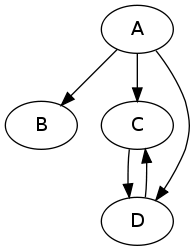
\includegraphics[width=1.4in]{figures/g1}
  \caption{Példa mérésből előálló gráf}
  \label{fig:g1}
\end{figure}
    
    \subsection{Megjelenítés}
    A feldolgozott adatok célja, hogy a karbantartó számára világossá tegye, hogy előfordulhat-e holtpont a mért alkalmazásban (azaz van-e két olyan szál, ami azonos erőforrásokon különböző zárolási sorrendet alkalmaz) és ha van, akkor segítse a karbantartó számára a problémás programrészek azonosítását. Ezen céloknak megfelelően a megjelenítés két részre oszlik.
    
    Egyrészről az alkalmazás biztosít egy gráfot (lásd~\ref{fig:g1}. ábra), mely az erőforrások zárolásának sorrendjét ábrázolja. 
    \begin{description}
        \item[Állítás:]Amennyiben a létrejövő gráf egy fa, a vizsgált erőforrások kölcsönös kizárást okozó zárolások nem juttatják holtpontra a mért alkalmazást.
        \item[Bizonyítás:]Indirekt módon. Tegyük fel, hogy az alkalmazást lemértük, nem jutott holtpontra, a mérés eredményeképpen előálló gráf egy fa és megfelelő időzítés esetén mégis előfordulhat holtpont. A holtpont kialakulásának feltétele az egymásra várás, vagyis T1 szál zárolta A erőforrást és vár B-re míg T2 szál zárolta B erőforrást és vár A-ra. Mivel más időzítési paraméterek mellett ez a két szál nem jutott holtpontra a mérés folyamán és sikeresen zárolták az erőforrásokat, az eredménygráf definíciója miatt A és B erőforrást reprezentáló csúcsok megjelennek és köztük irányított út található, tehát a gráfban kör van, tehát a gráf nem fa, így ellentmondásra jutunk.
    \end{description}
%    
    A felhasználó a mérés után ellenőrzi a gráfot; amennyiben az fa, az alkalmazás a fenti állításnak megfelelően a mért lefutás folyamán semmilyen időzítési paraméterek mellett nem futhat holtpontra, tehát nincs további módosításra szükség. Ha az eredménygráf nem fa, azaz tartalmaz irányított kört, akkor fennáll a holtpont előfordulásának veszélye, további vizsgálatra van szükség.
    
    Az érintett erőforrások vizsgálatát segíti a megjelenítést végző felület másik része. Az egyes erőforrásokat azonosító alapján -- mely megjelenik a gráf csúcsain -- kereshetjük ki a gyűjtött adatok közül, így képet kapva arról, hogy mely metódusok mentén történtek az egyes zárolások. A különböző zárolási hierarchiákat elemezve a karbantartó megállapíthatja, hogy melyik szál zársorrendje tekinthető \emph{hibásnak}, lokalizálva ezzel a módosítandó kódrészletet.
    
    \section{Implementáció}
    Az előzőekben a motivációra adott absztrakt választ részleteztem, kitérve a megoldás helyességének bizonyítására és értelmezésére, szorítkozva a feltétlenül szükséges logikai komponensekre, eltekintve az implementációs részletektől ott, ahol ez lehetséges volt. A következőkben az elkészített \emph{deadlockHunter} programot ismertetem először architekturális szinten, majd végigmegyek az egyes komponensek implementációs részletein, külön kiemelve a felmerülő kihívásokra adott válaszokat.
    
    \subsection{Architektúra}
    A fent specifikált alkalmazás megvalósítása architekturális szempontból két fő részt tesz szükségessé; Egy adatgyűjtésért és egy megjelenítésért felelős komponenst. A \emph{deadlockHunter} programban ez egy könyvtár (shared object) és egy bináris állomány formájában realizálódik. Az implementáció érdekessége, hogy a két komponens programkódja túlnyomó részben megegyezik. A \ref{fig:architecture}. ábra szemlélteti a komponensek kommunikációját.
    
\begin{figure}[ht!]
  \centering
    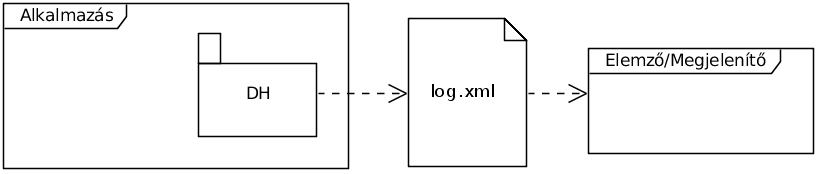
\includegraphics[width=5.4in]{figures/arch}
  \caption{Mérés komponenseinek lehetséges elrendezése}
  \label{fig:architecture}
\end{figure}    
%    
    A mérést végző komponens a gyűjtött adatokat vagy egy \texttt{XML} dokumentumba sorosítja, vagy Google Protocol Buffer\footnote{Google Protocol Buffer: https://developers.google.com/protocol-buffers} formátumba menti. A kinyert dokumentumot a megjelenítő komponens beolvassa és azokból egy gráfot készít valamint egy kereső felületet biztosít. A továbbiakban a két komponens jellemző részeit mutatom be röviden.
    
    \subsubsection{Google Protocol Buffer}
    Az \texttt{XML} formátum előnye, hogy karakteres természetéből adódóan ember számára is könnyen olvasható és kereshető, valamint gépi feldolgozása is egyszerű és számos platformon támogatott -- natív módon vagy könyvtárakon keresztül. Hátránya az \texttt{XML} formátumnak, hogy a dokumentum mérete a reprezentált információhoz képest nagyon nagy, amit körülményes tárolni és lassú beolvasni.
    
    A Google Protocol Buffer előnyei és hátrányai pont fordítottak. Azonos adatmennyiség sorosítás után sokkal kisebb méretű, mint \texttt{XML} esetében, a sorosított állomány beolvasása gyorsabb, viszont maga az állomány emberi olvasó számára értelmezhetetlen és az feldolgozás különböző platformokon külön támogatást és karbantartást igényel. Mivel jelen környezetben a kis méret és gyors feldolgozás abszolút prioritást élvez, a Protocol Buffer támogatás megjelenése után az \texttt{XML} formátum csupán tesztelési és kompatibilitási okokból van jelen a rendszerben.
    
    \subsection{Adatgyűjtés}
    Az adatgyűjtést úgy kellett megvalósítani, hogy a \emph{GlobalContractor} alkalmazásba könnyen integrálható legyen. A kódon végzett előzetes vizsgálat során kiderült, hogy minden kérdéses erőforrás -- többnyire rekurzív mutexek -- preprocesszor makrók egy szűk halmazának segítségével van zárolva és felszabadítva, a következő két idióma egyikével:
    
    \begin{description}
        \item[Guard idiom:] A makró egy osztályt példányosít a stacken. A konstruktor zárolja a megadott erőforrást, a blokk végére érve a stack lebontásakor pedig a destruktor felszabadítja azt. Ezt C++ környezetben \texttt{RAII} idiomnak nevezzük.
        \item[Acquire/Release idiom:] Külön makrók állnak rendelkezésre az erőforrás zárolására és felszabadítására, melyek az átadott címen található struktúrán hívnak előre definiált metódusokat (\texttt{acquire()} és \texttt{release()}).
    \end{description}
%    
    Láthatóan mindkét megoldás könnyen kibővíthető úgy, hogy a zárolás \emph{és} felszabadítás tényét egy külső megfigyelő felé jelezze, anélkül, hogy a makródefinícióktól eltekintve a mért rendszeren bármilyen változtatást kéne eszközölni. Az első idióma esetén egy további osztály példányosítása, a második esetben egy-egy metódus meghívása elegendő.
    
    A makrók újradefiniálását egy fordítási időben állítható kapcsolóhoz köthetjük, így az alkalmazás futásidejű terhelést kizárólag a mérés során szenved el, egyéb esetekben a teljesítmény a módosítatlan változattal megegyezik (mivel ugyan az a programkód kerül fordításra).

\medskip    
\lstset{
    basicstyle=\footnotesize\ttfamily
}    
    \lstinputlisting[language=C++]{figures/macro.cpp}
\medskip

\noindent    
Ezeket a jelzéseket fogadja a mérés során az alkalmazáshoz linkelt könyvtár. Minden szál szálspecifikus tárában (\emph{thread local storage}) elérhető egy egyke mintát követő (\emph{singleton}) osztály példánya, ami a jelzéseket tárolja. A szálspecifikus tároló használatának előnye, hogy az események regisztrálása során a versenyhelyzetek figyelmen kívül hagyhatóak (mivel minden szál saját memóriaterületét módosítja).
    
    Az egyes lokális tárolókat egy globális tároló fogja össze. Elsődleges feladata a mérés végén a gyűjtött adatok sorosítása és fájlba írása. Ezen globális példány felületén keresztül szükség esetén -- még a mérés futása közben is -- diagnosztikai információkhoz juthatunk (lásd Megjelenítés) valamint átmenetileg felfüggeszthetjük vagy újraindíthatjuk az adatgyűjtést.
    
    A \emph{GlobalContractor} alkalmazás esetében a mérés vezérlése egy adminisztrációs felületbe integrálódott.
    
    \subsection{Megjelenítés}
    A mérési eredmények analizálása és vizualizációja két különböző felületen keresztül történhet. Hagyományos parancssoros, valamint egy böngészőből elérhető grafikus felület áll rendelkezésre.
    
    Bármely klienst is válasszuk, a megjelenítés elsődleges feladata a mérés során előzőleg sorosított adatok beolvasása és értelmezése. A program a feldolgozott adatokból egy gráfot épít (az erőforrások azonosítására a memóriacíme szolgál), amiből egy \emph{Graphviz\footnote{Graphviz: gráf vizualizációs szoftver, http://www.graphviz.org/} .dot\footnote{DOT leírónyelv: http://www.graphviz.org/doc/info/lang.html}} formátumú struktúrát készít, ami alapján a \emph{Graphviz} program a gráfot ábrázoló képfájlokat képes előállítani. A program által biztosított formátumok közül érdemes az \texttt{svg} formátumot választani, és azt Mozilla Firefox böngészővel megtekinteni. Bármely más tesztelt kombináció (megjelenítés: Mozilla Firefox, Google Chrome, Microsoft Internet Explorer, Windows Image and Fax Viewer; formátumok: jpg, png, svg) elfogadhatatlan hibákat okozott a megjelenítésben, a képfájlok szokatlanul nagy mérete miatt (pl.: $20.000 * 5000$ pixel). A gráf egyes csúcsain megjelenő feliratok a csúcs által reprezentált erőforrást definiáló osztály neve található -- amit a program a kapcsolódó fájl neve alapján tippel meg -- egy egyedi azonosítóval kiegészítve, pl.: \texttt{ModelProxy.23}. Az osztály név megjelenítésére azért esett a választás, hogy a program futása a tapasztalt karbantartó számára könnyen követhető legyen. Az egyedi azonosítóra az egyes osztályok különböző példányaiban definiált -- különböző -- erőforrások megkülönböztetése miatt van szükség. A gráf élei szálanként különböző színnel vannak színezve, a színek és szálazonosítók összerendelése táblázatban jelenik meg a képen.
    
    \subsubsection{Parancssoros felület}
    
    A parancssoros felület a kötelező feladatain túl képes a kimeneti formátumok között konvertálni, valamint egy keresőfelületet biztosít, ami a gráfon megjelenített nevek alapján keres az elemzett adatok között, és megjeleníti a keresett erőforrásra jellemző zárolásokat és környezetüket, szálanként csoportosítva (\ref{fig:trace}. ábra). A szálak azonosítása platformfüggő. Linux platformon a szálhoz rendelt \texttt{LWP} jelenik meg. Ennek előnye, hogy a \emph{gdb} program ugyanezt az azonosítót használja, így -- például -- egy coredump elemzése során az egyes szálak könnyen azonosíthatóak.
    
    Az egyes események szöveges reprezentációja egy formátumsztring megadásával konfigurálható. A megjeleníthető mezők a következőek:

\begin{description}
    \item[\%t] Esemény típusa (zárolás vagy felszabadítás)
    \item[\%f] Eseményt kiváltó metódus neve (GCC fordító használata esetén a \\ \texttt{\_\_PRETTY\_FUNC\_\_} kiegészítés használatával)
    \item[\%F] Kiváltó utasítást tartalmazó fájl neve
    \item[\%l] Kiváltó utasítást tartalmazó sor száma
    \item[\%a] Erőforrás memóriacíme
\end{description}

\noindent     
Az egyes mezők tetszőlegesen kombinálhatóak és kiegészíthetőek más karakterekkel.
    
\begin{figure}[ht!]
    \noindent
    \texttt{Thread \#12345 \\
    \\
    > lockFirst() (App.cc:186) \\
    \hspace*{8pt}    > lockSecond() (App.cc:219) [*]\\
    \hspace*{8pt}    < lockSecond() (App.cc:219) [*]\\    
    < lockFirst() (App.cc:186) \\
    \\
    Thread \#54321 \\
    \\
    > lockSecond() (App.cc:219) [*]\\
    \hspace*{8pt}    > lockFirst() (App.cc:186) \\
    \hspace*{8pt}    < lockFirst() (App.cc:186) \\
    < lockSecond() (App.cc:219) [*]\\
    }
  \caption{Keresés eredménye (példa). A *-al jelölt sorok a keresett erőforrásra vonatkozó események}
  \label{fig:trace}
\end{figure}

    \subsubsection{Grafikus felület}
    A parancssori felület megvalósítása egyszerű, a működése a lehető leggyorsabb, keresztplatformos megoldás, viszont rendelkezik néhány komoly hátránnyal is: a platformfüggetlen folyamkezlés miatt nem támogatja a kurzorbillentyűk kezelését, az automatikus parancs kiegészítést, valamint a használata nem intuitív. A problémák megoldása végett elkészítettem egy grafikus felületet, ami böngészőből érhető el.
    
    A működéshez szükség volt egy http szerverre, ami képes kommunikálni a C++ kódbázissal, elérhető a vállalati környezetben, pehelysúlyú és egyszerűen integrálható. A számbavett alternatívák a következőek:
    
\begin{description}
    \item[Mongoose:\footnotemark] \footnotetext{C++ nyelvű webszerver: https://github.com/valenok/mongoose}Kis méretű, egyszerű C++ szoftver, ami így nagyszerű választás lenne, de sajnos nem elérhető a vállalton belül.
    \item[Twisted:\footnotemark] \footnotetext{Python nyelvű esemény orientált hálózati motor: http://twistedmatrix.com/} Kiforrott, stabil szoftver, szimpatikus szkriptnyelv; viszont nem találtam olyan Python/C++ interoperabilitási lehetőséget, ami megfelelt volna a követelményeknek.
    \item[Node.js:\footnotemark] \footnotetext{Javascript nyelvű hálózati platform: http://nodejs.org/} A követelményeket legnagyobb részben kielégíti és volt már tapasztalatom a szükséges felhasználási móddal. A Javascript/C++ integráció nem triviális és nagyon törékeny, lásd később.
   
\end{description}
%    
    A fentiek alapján a választás a Node.js-re esett. A Javascript/C++ kommunikáció megvalósítása végett készítettem egy Node.js \emph{addont}, ami a beérkező kéréseket továbbítja a C++ komponensnek, a választ pedig Javascript objektumok formájában teszi elérhetővé. Az integráció a Node.js által használt Google V8 Javascript motoron\footnote{Google V8 Javascript motor: http://code.google.com/p/v8/} alapul.
   
    Ezentúl írtam egy Node.js szerver programot Javascript nyelven, ami kiszolgálja az -- automatikusan elkészített, -- a mérést reprezentáló gráfot, lehetővé teszi a zárolási események kényelmes keresését, a szálak aggregált információinak megtekintését, valamint biztosít egy \emph{intelligens trace} funkciót.
    
    A keresési kifejezésre illeszkedő rögzített eseményeket listázó oldalon megjelenő kontextusok sora adott esetben hosszúra nyúlhat, és dacára minden optimalizációnak, többnyire egy erőforrásra vonatkozóan hasonló részleteket mutat, amelyek közül körülményes kikeresni az érdekes mintákat. A leggyakoribb feladat olyan minták keresése, ahol két erőforrás mindkét lehetséges sorrendben lefoglalásra kerül. A kérdéses erőforrások azonosítása lehetővé válik az eredménygráf vizsgálatával. A körök azonosításnak lehetőségét Tarjan erősen összefüggő komponensek algoritmusa és egy saját rekurzív konstrukció biztosítja. Az \emph{Autotrace} funkció az így kapott és érdekesnek ítélt, konfliktusos szálak releváns erőforrás kontextusait listázza.
    
    A felület használatához el kell indítani egy lokális Node.js szervert (\texttt{\$ node server.js}), ezután a konzolon megjelenő címen az alkalmazás elérhető. Az eredmények analizálása során a böngészett tartalmat egyértelműen azonosítja az URL-je, valamint egyes -- érdekesnek tartott -- részek külön meg is jelölhetőek, mely jelölések tükröződnek az URL-ben; így a karbantartó a fontos eredményeket egyszerűen meg tudja osztani kollégáival a linket továbbküldve. A felület funkcionalitásáért jQuery\footnote{jQuery: kliens oldalra szánt Javascript keretrendszer: http://jquery.com/}, az igényes megjelenéséért Twitter Bootstrap\footnote{Twitter Bootsrap frontend keretrendszer: http://twitter.github.com/bootstrap/} keretrendszerek felelnek.
    
    Az így kapott felület intuitív, valamint az eléréséhez csupán egy böngészőre van szükség. A megoldás hátránya, hogy a Javascript/C++ átmenetért felelős illesztő komponens lefordításához rendelkeznünk kell a megfelelő Node.js könyvtárakkal (\emph{shared object}), amiket ugyanazzal a fordítóval lettek fordítva.

    \section{Optimalizálás}
    A \emph{deadlockHunter} a fent leírt formában funkcionálisan késznek tekinthető, azonban használhatóság téren a gyakorlatban kívánnivalókat hagy maga után. A kezdeti tesztelések megmutatták, hogy egy igazán komplex alkalmazás hosszas mérése komoly teljesítménybeli problémákat okozhat. A konkrét problémákat a következő alfejezetekben ismertetem a megoldásaikkal együtt. Amikor ezek a problémák felmerültek, a kiutat nem a kód mikrooptimalizálásában kerestem, -- egy-egy gépi utasítás megspórolása itt-ott nem segített volna -- hanem az adatstruktúrák és algoritmusok javításában. Ennek megfelelően aprólékos kódoptimalizálásra nem került sor, mivel nem volt rá szükség.
    
    \subsection{Az adatgyűjtés optimalizálása}
    
Az egyik problémát a mérés folyamán az események válogatás nélküli regisztrálása jelentette. A mért alkalmazásban gyakran előfordult a következő minta: Egy nagy elemszámú listán iterált, minden elem feldolgozása előtt az elemet zárolta egy megfelelő mutexen keresztül, majd a feldolgozás végeztével a zárat elengedte. Ez sok esemény bejegyzését jelentette. Mivel ezeket az iterációkat az alkalmazás minden gerjesztés mellőzése esetén, "üresjáratban" is folytatta, a tárolt események száma nagyon gyorsan növekedett, hamar túllépve a rendelkezésre álló memóriát (A tesztkörnyezetben 16 GB-ot).

    A triviális megoldása a problémának, hogy a tárolt események számának függvényében azokat időnként a háttértárra mentjük és a memóriából eltávolítjuk. Ennek a megközelítésnek több hátulütője is van: Továbbra is rengeteg eseménnyel kell majd foglalkozi a megjelenítés során, ami ott újabb teljesítményproblémákhoz vezethet, a hatalmas kimeneti fájlok kezelése nehézkes és archiválásuk költséges valamint a folyamatos fájlműveletek feleslegesen lassítják a mérést.
    
    Egy jobb megoldáshoz jutunk, ha a fent említett mintát figyeljük meg. A ciklus ismételt futtatása újból és újból ugyan azokat az eseménysorokat eredményezi. Egyszerűen adódna, hogy akkor ezeket az ismétléseket csoportosítsuk, és spóroljuk meg például az ismétlődő stringek tárolását egy string cache használatával. Ez egy életképes elgondolás, azonban az eseménycsoportok összehasonlítása újabb felismeréshez vezet el: Kizárólag az időzítési paramétereikben különböznek, vagyis egy olyan jellemzőben, amit szándékosan nem veszünk figyelembe mivel a gráfalkotás során ez az információ eldobásra kerül. Tehát az egyes eseménycsoportok közül egy tetszőleges kivételével a többi eldobható, anélkül, hogy veszítenénk a mérés pontosságából.
    
    Ennek megfelelően az eseményeket regisztráló komponens a következő képpen változik:
    
    \begin{enumerate}
        \item Kezdetben egy üres csoportlistával és egy üres átmeneti listával jön létre
        \item A beérkező eseményeket az átmeneti listában rögzíti
        \item A csoport végén az átmeneti listát összehasonlítja az összes eddigi csoporttal. Ha talál olyan csoportot, amely megegyező sorrendben tartalmaz az átmeneti csoportban található eseményekkel ekvivalens eseményeket, és csak azokat, akkor az átmeneti listát eldobja, és újat kezd. Egyébként az átmeneti listát elmenti új csoportként, és ezután üríti.
    \end{enumerate}
    
    Hogy a megoldás működhessen két fogalmat kell definiálni: Mikor van egy csoportnak vége, valamint mikor mondunk két eseményt ekvivalensnek. Mindkét fogalom nagyon komolyan befolyásolja a mérés kimenetelét, a definíciókat úgy határoztam meg, hogy azok segítsék a \emph{GlobalContractor} mérését. Más alkalmazás esetén előfordulhat, hogy egy alkalmasabb definíció található.
    
    A csoportok határának meghatározására a szál által zárva tartott erőforrások számát használtam fel. Ehez nyilván kell tartani a mérőszámot, ami konstans időben megtehető. Amennyiben a zárolt erőforrások száma elér egy előre meghatározott korlátot, az aktuális csoport lezárásra kerül. A korlátot alkalmasan kell megválasztani, a gyakori minták függvényében. A \emph{GlobalContractor} esetében ezt a korlátot a 0 szinten határoztam meg. Amennyiben egy szál elenged minden erőforrást, zárolódik az addigi tevékenysége. (Ez a választás elősegítette azt is, hogy a csoportok használata egy teljesen más helyzetben nyújtson segítséget) Ha előfordul, hogy egy szál futásának kezdetén magához ragad egy erőforrást, és azt hosszú időn keresztül nem engedi el, miközben sok különböző tevékenységet hajt végre -- sok eseményt generál -- akkor megfontolandó a korlát felemelése, hogy az így kialakuló nagyméretű csoportokat feldaraboljuk. Ennek ára van, 0-tól különböző korlát használata további óvintézkedéseket igényel, egy esetleges hibás mérést megelőzendő.
    
    Az egyes események közötti egyenlőség operátor definiálása során ugyancsak érdemes figyelembe venni az alkalmazás jellegzetességeit. Amennyiben ezt nem tesszük meg, a válasz triviálisan adódik: Két esemény megegyezik, ha minden róla tárolt információ megegyezik (pl.: fájl, sor és memóriacím). Ez a választás helyességét tekintve megfelelő, viszont a kritérium relaxálásával könnyebben feldolgozható eredményt kapunk. Bizonyos esetekben előfordulhat, hogy megengedhejük a memóriacím különbözőségét (és csak a fájlt valamint a sort ellenőrizzük). Ez a választás a legtöbb esetben nem helyes, viszont alkalmanként mégis jó és könnyen elemezhető gráfhoz vezet minket, amin jobban megfigyelhetőek az egyes zárolási minták.
    
    A \emph{GlobalContractor} esetében, más optimalizációk használata mellett a választás a fájl nevét, a forráskód sorszámát és az erőforrás memóriacímét figyelembe vevő egyenlőség operátorra esett.
    
    Az optimalizáció megvalósítását követően a mérőkóddal ellátott alkalmazás memóriahasználata alig tért el az alapértelmezett működés közben megfigyelhető igényektől, és üresjáratban semmilyen emelkedést nem mutatott, így teljes mértékben elérte célját.
    
    % \subsection{Az adatgyűjtés optimalizálásának teljesítménymérése}
    % Too much effort required -- skip
    
    \subsection{A megjelenítés optimalizálása}
    Egy kiterjedt teszt futtatása -- még a fenti optimalizáció figyelembe vételével is --nagyon sok regisztrált eseményhez vezet, ami a gráf reprezentációt áttekinthetetlenné teszi. A probléma forrása, hogy olyan események is megjelennek, amelyek nem vesznek részt holtpont kialakításában. Az ilyen eseményeket reprezentáló csúcsokat eltüntethetjük, ha az eredménygráf levél csúcsainak levágását addig ismételjük, amíg van ilyen csúcs.
    
    \begin{description}
        \item[Állítás:] A gráf leveleinek ismételt levágásával nem veszítünk el lehetséges holtpontra utaló mintát.
        \item[Bizonyítás:] Korábban beláttuk, hogy a gráf konstrukciója miatt csak akkor alakulhat ki holtpont az alkalmazásban, ha az irányított gráf nem fa, vagyis ha irányított kört tartalmaz. Tehát amíg nem vágunk le olyan csúcsot, ami egy irányított kör eleme, addig nem veszítünk el értékes információt sem. Mivel egy csúcs pontosan akkor levél, ha nincs belőle kimenő irányított él, ezért egy levél nem lehet irányított kör eleme, tehát elhagyható. Mivel az így keletkező gráf pontosan ugyan azt az értékes információt hordozza, mint az előző, a lépést megismételhetjük, egészen addig, amíg van levél csúcs.
        \item[Megjegyzés:] Ha az eredménygráf fa, az összes csúcsot eldobhatjuk és üres gráfot kapunk -- tehát holtpontra nincs lehetőség -- ami megfelel a korábbi állításnak.
    \end{description}
%    
    Az így kapott, jelentősen redukált méretű gráf sokkal könnyebben elemezhető, ám egy -- az előzőhöz nagyon hasonló -- ötlettel még több csúcsot hagyhatunk el.
    
    \begin{description}
        \item[Állítás:] A gráf gyökér csúcsainak ismételt levágásával nem veszítünk el lehetséges holtpontra utaló mintát.
        \item[Bizonyítás:] Az előző mintájára. Egy csúcs pontosan akkor gyökér, ha nem mutat rá irányított él, tehát nem mehet át rajta irányított kör, vagyis eldobható. Az értékes információ megmaradása miatt a lépés ismételhető, amíg van gyökér pont.
        \item[Megjegyzés:] Az előző módszerhez hasonlóan, csak ezt az eljárást alkalmazva pontosan akkor lesz a kimeneti gráf az üres gráf, ha a bemeneti gráf fa volt.
        \item[Megjegyzés 2:] A módszert alkalmazva a gráf elveszítheti összefüggőségét.
    \end{description}
%    
    A bemutatott két módszerrel transzformált gráf nagyságrendekkel kevesebb csúcsot tartalmazott a \emph{GlobalContractor} esetében és emberi vizsgálatra sokkal alkalmasabbnak bizonyult. Tekintve, hogy a fenti tételek szerint információt nem veszítettünk, az optimalizáció hasznosnak ítélhető.
    
    \section{Fejlesztési tervek}
    A \emph{deadlockHunter} jelen formájában használható és betölti a célját, viszont a fejlesztés és tesztelés során felmerültek további ötletek, melyek növelnék a felhasználóbarátságot vagy a project fejlődése miatt fontosak. Az örökös fejlődés igénye egy szoftver sajátja és szerves része, ezért ezen ötletek közül a következőkben ismertetem a legfontosabbakat.
    
    \subsection{Forráskód megnyitása}
    A project nem jöhetett volna létre a fejlesztés során használt számtalan nyílt forráskódú szoftver nélkül (pl.: Linux, GCC, Eclipse, git, boost, graphviz és mások), így egyértelmű a forrás megnyitásának motivációja, tekintve továbbá, hogy az eszköz általános célú, így más környezetben is hasznosnak bizonyulhat.
    
    A \emph{deadlockHunter} már nem tartalmaz vállalati (\emph{proprietary}) függőségekket, azokat lecseréltem funkcionálisan ekvivalens, nyílt forráskódú alternatíváikra. Az utolsó lépés, hogy a forráskód megnyitását a Morgan Stanley megfelelő testülete is jóváhagyja. Az erőfeszítés sikeressége egyelőre bizonytalan, de valószínűsíthető. Amennyiben az akció sikerrel jár, az eszköz szabadon elérhetővé tétele az eddigi gyakorlattól eltérő, egyedülálló esemény lesz a vállalat történetében, és remélhetőleg egy új irány kezdete.
    
    \subsection{Felhasználói dokumentáció készítése}
    Ha sikerül a forráskód megnyitása, szükségessé válik egy mindenki számára szabadon elérhető dokumentáció elkészítése is, mely tartalmazz felhasználói segédletet és integrátori útmutatót is. Mivel jelen dokumentum a teljesség igényével részletezi az alkalmazás fontos részeit, nem alkalmas a felhasználói dokumentáció szerep betöltésére.
    
    \subsection{Újrafordítás nélküli felhasználás}
    A jelenlegi változat preprocesszor makrókat használ a megfigyelendő függvényhívások monitorozhatóvá tétele érdekében. Ez a megoldás a teljes alkalmazás újrafordítását igényli a mérőeszköz be- és kikapcsolása esetén. A váltás felgyorsítása érdekében elérhetővé kell tenni egy olyan monitor megoldást, melynek bekapcsolása dinamikus linkelési időben történik, Unix szerű rendszereken az \texttt{LD\_PRELOAD}\footnote{https://en.wikipedia.org/wiki/LD\_PRELOAD} környezeti változó által biztosított felületen, míg Windows rendszereken a \emph{DLL Injection}\footnote{https://en.wikipedia.org/wiki/DLL\_Injection} megoldáson keresztül.
    
    \subsection{Automatikus kiegészítés a keresőben}
    A grafikus felületet az egyszerűbb és kényelmesebb használat érdekében kell úgy továbbfejleszteni, hogy a keresőben megjelenjenek a lehetséges, illeszkedő keresőkifejezések, automatikus kiegészítés formájában. Ehhez meg kell teremteni a lehetőséget, hogy a C++ oldal kiajánlja a rendelkezésre álló opciókat.
    
    \subsection{Kódtisztítás}
    A C++ programkódon elvégzendő néhány apró, de átfogó változtatás:

    \begin{description}
        \item[Dokumentáció:] Ahol esetleg még hiányzik az API dokumentáció, ott azt el kell készíteni, valamint az összes API dokumentációt át kell nézni és az esetlegesen elavult részeket frissíteni kell. Ezután a forráskódból különálló dokumentációt kell generálni, az automatizmust rögzítve, megismételhető módon.
        
        \item[Projekt namespace:] Az integráció egyszerűsítése végett az összes komponenst egy közös \texttt{namespace} alá kell helyezni.
        
        \item[Guard macro nevek:] A fejléc fájlok \emph{guard macro}i jelenleg a következő formátumban vannak: \texttt{\_CLASSNAME\_H}. Ezt kell átalakítani úgy, hogy tükrözze a könyvtárstruktúrát.

    \end{description}
